\begin{figure}[H]
	\centering
	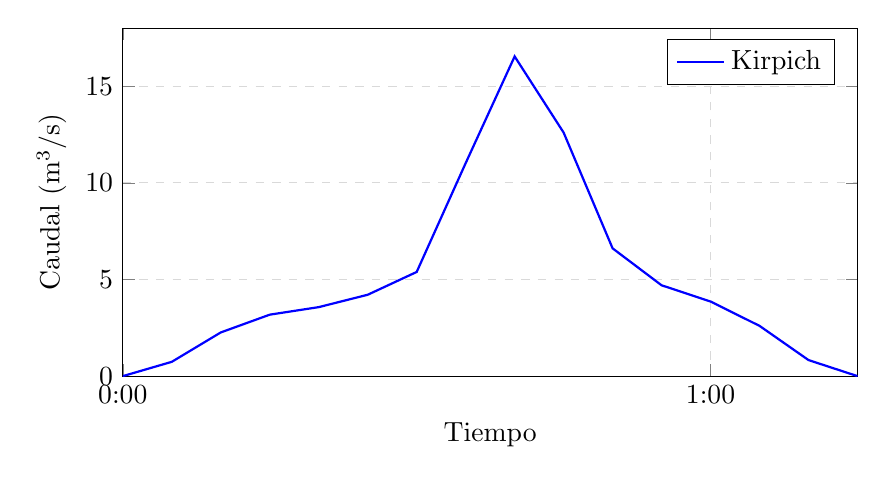
\begin{tikzpicture}
		\begin{axis}[
			width=0.9\textwidth,
			height=6cm,
			xlabel={Tiempo},
			ylabel={Caudal (m$^3$/s)},
			xmin=0,
			xmax=75,
			ymin=0,
			ymax=18,
			grid=major,
			grid style={dashed, gray!30},
			legend pos=north east,
			xtick={0, 60},
			xticklabels={0:00, 1:00},
			]
		% Kirpich
		\addplot [
		blue,
		thick,
		solid,
		] coordinates {
				(0, 0.00) (5, 0.74) (10, 2.26) (15, 3.18) (20, 3.57)
				(25, 4.21) (30, 5.39) (35, 11.02) (40, 16.54) (45, 12.60)
				(50, 6.61) (55, 4.70) (60, 3.86) (65, 2.60) (70, 0.83)
				(75, 0.00)
		};
		\addlegendentry{Kirpich}

		\end{axis}
	\end{tikzpicture}
	\caption{Hidrograma - Kirpich + BLOCKS $T_r$=25 años ($Q_p$=16.541 m$^3$/s)}
	\label{fig:hydro_kirpich_blocks_Tr25}
\end{figure}
